%% BioMed_Central_Tex_Template_v1.06
%%                                      %
%  bmc_article.tex            ver: 1.06 %
%                                       %

%%IMPORTANT: do not delete the first line of this template
%%It must be present to enable the BMC Submission system to
%%recognise this template!!

%%%%%%%%%%%%%%%%%%%%%%%%%%%%%%%%%%%%%%%%%
%%                                     %%
%%  LaTeX template for BioMed Central  %%
%%     journal article submissions     %%
%%                                     %%
%%          <8 June 2012>              %%
%%                                     %%
%%                                     %%
%%%%%%%%%%%%%%%%%%%%%%%%%%%%%%%%%%%%%%%%%


%%%%%%%%%%%%%%%%%%%%%%%%%%%%%%%%%%%%%%%%%%%%%%%%%%%%%%%%%%%%%%%%%%%%%
%%                                                                 %%
%% For instructions on how to fill out this Tex template           %%
%% document please refer to Readme.html and the instructions for   %%
%% authors page on the biomed central website                      %%
%% http://www.biomedcentral.com/info/authors/                      %%
%%                                                                 %%
%% Please do not use \input{...} to include other tex files.       %%
%% Submit your LaTeX manuscript as one .tex document.              %%
%%                                                                 %%
%% All additional figures and files should be attached             %%
%% separately and not embedded in the \TeX\ document itself.       %%
%%                                                                 %%
%% BioMed Central currently use the MikTex distribution of         %%
%% TeX for Windows) of TeX and LaTeX.  This is available from      %%
%% http://www.miktex.org                                           %%
%%                                                                 %%
%%%%%%%%%%%%%%%%%%%%%%%%%%%%%%%%%%%%%%%%%%%%%%%%%%%%%%%%%%%%%%%%%%%%%

%%% additional documentclass options:
%  [doublespacing]
%  [linenumbers]   - put the line numbers on margins

%%% loading packages, author definitions

%\documentclass[twocolumn]{bmcart}% uncomment this for twocolumn layout and comment line below
\documentclass{bmcart}

%%% Load packages
%\usepackage{amsthm,amsmath}
%\RequirePackage{natbib}
%\RequirePackage{hyperref}
\usepackage[utf8]{inputenc} %unicode support
%\usepackage[applemac]{inputenc} %applemac support if unicode package fails
%\usepackage[latin1]{inputenc} %UNIX support if unicode package fails
\usepackage{graphicx}

\renewcommand*{\thefootnote}{\fnsymbol{footnote}}

%%%%%%%%%%%%%%%%%%%%%%%%%%%%%%%%%%%%%%%%%%%%%%%%%
%%                                             %%
%%  If you wish to display your graphics for   %%
%%  your own use using includegraphic or       %%
%%  includegraphics, then comment out the      %%
%%  following two lines of code.               %%
%%  NB: These line *must* be included when     %%
%%  submitting to BMC.                         %%
%%  All figure files must be submitted as      %%
%%  separate graphics through the BMC          %%
%%  submission process, not included in the    %%
%%  submitted article.                         %%
%%                                             %%
%%%%%%%%%%%%%%%%%%%%%%%%%%%%%%%%%%%%%%%%%%%%%%%%%


%\def\includegraphic{}
%\def\includegraphics{}



%%% Put your definitions there:
\startlocaldefs
\endlocaldefs


%%% Begin ...
\begin{document}

%%% Start of article front matter
\begin{frontmatter}

\begin{fmbox}
\dochead{Commentary}

%%%%%%%%%%%%%%%%%%%%%%%%%%%%%%%%%%%%%%%%%%%%%%
%%                                          %%
%% Enter the title of your article here     %%
%%                                          %%
%%%%%%%%%%%%%%%%%%%%%%%%%%%%%%%%%%%%%%%%%%%%%%

\title{Ten recommendations for software engineering in research}

%%%%%%%%%%%%%%%%%%%%%%%%%%%%%%%%%%%%%%%%%%%%%%
%%                                          %%
%% Enter the authors here                   %%
%%                                          %%
%% Specify information, if available,       %%
%% in the form:                             %%
%%   <key>={<id1>,<id2>}                    %%
%%   <key>=                                 %%
%% Comment or delete the keys which are     %%
%% not used. Repeat \author command as much %%
%% as required.                             %%
%%                                          %%
%%%%%%%%%%%%%%%%%%%%%%%%%%%%%%%%%%%%%%%%%%%%%%

\author[
   addressref={aff1},                   % id's of addresses, e.g. {aff1,aff2}
   corref={aff1},                       % id of corresponding address, if any
   email={hastings@ebi.ac.uk}   % email address
]{\inits{JH}\fnm{Janna} \snm{Hastings}}
\author[
   addressref={aff1},
   email={kenneth@ebi.ac.uk}
]{\inits{KH}\fnm{Kenneth} \snm{Haug}}
\author[
   addressref={aff1},
   email={steinbeck@ebi.ac.uk}
]{\inits{CS}\fnm{Christoph} \snm{Steinbeck}}

%%%%%%%%%%%%%%%%%%%%%%%%%%%%%%%%%%%%%%%%%%%%%%
%%                                          %%
%% Enter the authors' addresses here        %%
%%                                          %%
%% Repeat \address commands as much as      %%
%% required.                                %%
%%                                          %%
%%%%%%%%%%%%%%%%%%%%%%%%%%%%%%%%%%%%%%%%%%%%%%

\address[id=aff1]{%                           % unique id
  \orgname{Cheminformatics and Metabolism, European Molecular Biology Laboratory -- European Bioinformatics Institute}, % university, etc
  \street{Wellcome Trust Genome Campus},                     %
  %\postcode{}                                % post or zip code
  \city{Hinxton},                              % city
  \cny{UK}                                    % country
}

%%%%%%%%%%%%%%%%%%%%%%%%%%%%%%%%%%%%%%%%%%%%%%
%%                                          %%
%% Enter short notes here                   %%
%%                                          %%
%% Short notes will be after addresses      %%
%% on first page.                           %%
%%                                          %%
%%%%%%%%%%%%%%%%%%%%%%%%%%%%%%%%%%%%%%%%%%%%%%

\begin{artnotes}
%\note{Sample of title note}     % note to the article
%\note[id=n1]{Equal contributor} % note, connected to author
\end{artnotes}

\end{fmbox}% comment this for two column layout

%%%%%%%%%%%%%%%%%%%%%%%%%%%%%%%%%%%%%%%%%%%%%%
%%                                          %%
%% The Abstract begins here                 %%
%%                                          %%
%% Please refer to the Instructions for     %%
%% authors on http://www.biomedcentral.com  %%
%% and include the section headings         %%
%% accordingly for your article type.       %%
%%                                          %%
%%%%%%%%%%%%%%%%%%%%%%%%%%%%%%%%%%%%%%%%%%%%%%

\begin{abstractbox}

\begin{abstract} % abstract
%\parttitle{First part title} %if any
Research in the context of data-driven science requires a backbone of well-written software, but scientific researchers are typically not trained at length in software engineering, the principles for creating better software products. To address this gap, in particular for young researchers new to programming, we give ten recommendations to ensure the usability, sustainability and practicality of research software. 

%\parttitle{Second part title} %if any
%Text for this section.
\end{abstract}

%%%%%%%%%%%%%%%%%%%%%%%%%%%%%%%%%%%%%%%%%%%%%%
%%                                          %%
%% The keywords begin here                  %%
%%                                          %%
%% Put each keyword in separate \kwd{}.     %%
%%                                          %%
%%%%%%%%%%%%%%%%%%%%%%%%%%%%%%%%%%%%%%%%%%%%%%

\begin{keyword}
\kwd{software engineering}
\kwd{best practices}
\end{keyword}

% MSC classifications codes, if any
%\begin{keyword}[class=AMS]
%\kwd[Primary ]{}
%\kwd{}
%\kwd[; secondary ]{}
%\end{keyword}

\end{abstractbox}
%
%\end{fmbox}% uncomment this for twcolumn layout

\end{frontmatter}

%%%%%%%%%%%%%%%%%%%%%%%%%%%%%%%%%%%%%%%%%%%%%%
%%                                          %%
%% The Main Body begins here                %%
%%                                          %%
%% Please refer to the instructions for     %%
%% authors on:                              %%
%% http://www.biomedcentral.com/info/authors%%
%% and include the section headings         %%
%% accordingly for your article type.       %%
%%                                          %%
%% See the Results and Discussion section   %%
%% for details on how to create sub-sections%%
%%                                          %%
%% use \cite{...} to cite references        %%
%%  \cite{koon} and                         %%
%%  \cite{oreg,khar,zvai,xjon,schn,pond}    %%
%%  \nocite{smith,marg,hunn,advi,koha,mouse}%%
%%                                          %%
%%%%%%%%%%%%%%%%%%%%%%%%%%%%%%%%%%%%%%%%%%%%%%

%%%%%%%%%%%%%%%%%%%%%%%%% start of article main body
% <put your article body there>

%%%%%%%%%%%%%%%%
%% Background %%
%%
\section*{Background}

Scientific research increasingly harnesses computing as a platform \cite{goble2014}, and the size, complexity, diversity and relatively high availability of research datasets in a variety of formats is a strong driver to deliver well-designed, efficient and maintainable software and tools.
As the frontier of science evolves, new tools constantly need to be written. However, scientists (particularly hands-on early-career researchers) might not have received training in software engineering \cite{wilson2014bestpractice}, thus their code risks being difficult and costly to maintain and re-use. 

To address this gap, we have compiled ten brief software engineering recommendations. 

\section*{Recommendations}

\subsection*{1. Keep It Simple}

Every software project starts somewhere. A rule of thumb is to \textit{start as simply as you possibly can}. Significantly more problems are created by over-engineering than under-engineering. Simplicity starts with design: a clean\footnote{http://java.dzone.com/articles/what-clean-code-\%E2\%80\%93-quotes} and elegant data model is a kind of simplicity that leads naturally to efficient algorithms.  
 
Do the simplest thing that could possibly work, and then double-check it really does work. 

\subsection*{2. Test, Test, Test}

For objectivity, large software development efforts assign different people to test software than those who develop it. This is a luxury not available in most research labs, but there are robust testing strategies available to even the smallest project. 

Unit tests are software tests which are executed automatically on a regular basis. In test \textit{driven} development, the tests are written first, serving as a specification and checking every aspect of the intended functionality as it is developed \cite{tdd}. Make sure that unit tests exhaustively simulate \textit{all possible} -- not only that which seems reasonable -- inputs to each method. 

\subsection*{3. Don't Repeat Yourself}

Don't be tempted to use the copy-paste-modify coding technique when you encounter similar requirements. Even though this \textit{appears} the simplest approach, it won't remain simple, because important lines of code will end up duplicated. When making changes, you'll have to do them twice, taking twice as long, and you may forget an obscure place to which you copied that code, leaving a bug. 

Automated tools such as Simian\footnote{http://www.harukizaemon.com/simian/} can help to detect and fix duplication in existing codebases. To fix, consider writing a library with methods that can be called when needed.  

\subsection*{4. Use A Modular Design}

Modules act as building blocks that can be glued together to achieve overall system functionality. They hide the details of their implementation behind a public interface, which provides all the methods that should be used. Users should code -- and test -- to the interface rather than the implementation \cite{effectivejava2008}. Thus, concrete implementation details can change without impacting downstream users of the module. APIs (application programming interfaces) can be shared between different implementation providers. 

Scrutinise modules and libraries that already exist for the functionality you need. Don't rewrite what you can profitably re-use -- and don't be put off if the best candidate third-party library contains more functionality than you need (now).  

\subsection*{5. Involve Your Users}

Users know what they need software to do. Let them try the software as early as possible, and make it easy for them to give feedback, via a mailing list or an issue tracker. In an open source software development paradigm, your users can become co-developers. In closed-source and commercial paradigms, you can offer early-access beta releases to a trusted group.  

Many sophisticated methods have been developed for user experience analysis. For example, you could hold an interactive workshop \cite{pavelin2014}. 

But beware: sometimes, users ask for too much (feature creep). 

\subsection*{6. Resist Gold Plating}

Learn to tell the difference between essential features and the long list of wishes users may have. Prioritise aggressively and with as broad a collection of stakeholders as possible, perhaps using ``game-storming'' techniques \cite{gamestorm}.   

Gold plating is a challenge in all phases of development, not only in the early stages of requirements analysis. In its most mischievous disguise it appears as slow scope creep where just a little something is added in every iterative project meeting. Those little somethings add up. 

\subsection*{7. Document Everything}

Comprehensive documentation helps other developers who may take over your code, and also helps the future you. Use code comments for in-line documentation, especially for any technically challenging blocks, and public interface methods. However, there is no need for comments that mirror the exact detail of code line-by-line. 

It is better to have two or three lines of code that are easy to understand than to have one incomprehensible line (e.g. Figure~\ref{fig-incomprehensible}). 

%\begin{figure}%
%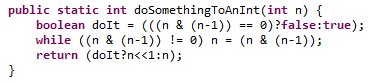
\includegraphics[width=\columnwidth]{code-snippet.png}%
%\caption{An example of incomprehensible code: What does this code actually do? It contains a bug; is it easy to spot?}%
%\label{fig-incomprehensible}%
%\end{figure}

Write clean code \cite{cleancode} that \textit{you} would \textit{want} to maintain long-term (e.g. Figure~\ref{fig-comprehensible}). Meaningful, readable variable and method names are a form of documentation. 

%\begin{figure}%
%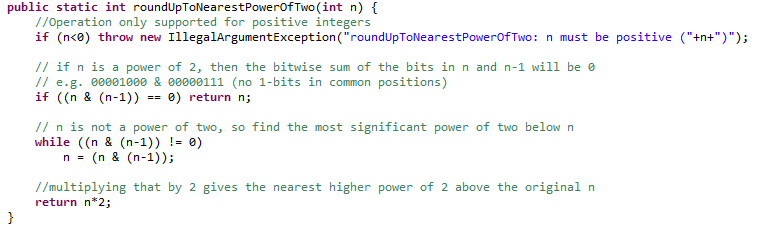
\includegraphics[width=\columnwidth]{code-snippet-fixed.png}%
%\caption{This code peforms the same function, but is written more clearly.}%
%\label{fig-comprehensible}%
%\end{figure}

Write an easily accessible module guide for each module, explaining the higher level view: what is the purpose of this module, how it fits together with other modules, and how to get started using it. 

\subsection*{8. Avoid Spaghetti}

Since GOTO-like commands fell justifiably out of favour several decades ago \cite{dijkstra1968}, you might believe that spaghetti code is a thing of the past. However, a similar phenomenon may be observed in inter-method and inter-module relationships (see Figure~\ref{fig-spaghetti},\ref{fig-not-spaghetti}). Debugging -- stepping through your code as it executes line by line -- can help you diagnose modern-day spaghetti code. Beware module designs where for every unit of functionality you have to step through several different modules to discover where the error is, and along the way you've long lost the record of what the original method was actually doing or what the erroneous input was. The use of effective and granular logging is another way to trace and diagnose problems with the flow through code modules. 

%\begin{figure}%
%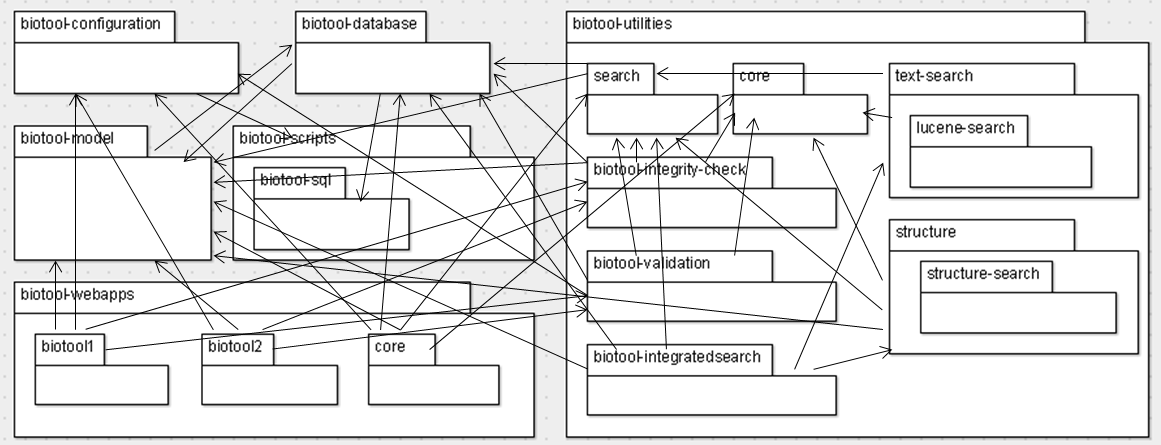
\includegraphics[width=\columnwidth]{ComplexClassDiagram.png}%
%\caption{An unhealthy module design for `biotool` with multiple interdependencies between different packages. An addition of functionality to the system (such as supporting a new field) requires updating the software in many different places. Refactoring into a simpler architecture would improve maintainability.}%
%\label{fig-spaghetti}%
%\end{figure}

\subsection*{9. Optimise Last}

Beware optimising too early. Although research applications are often performance-critical, until you truly encounter the wide range of inputs that your software will eventually run against in the production environment, it may not be possible to anticipate where the real bottlenecks will lie. Develop the correct functionality first, deploy it and then continuously improve it using repeat evaluation of the system running time as a guide (while your unit tests keep checking that the system is doing what it should). 

\subsection*{10. Evolution, Not Revolution}

Maintenance becomes harder as a system gets older. Take time on a regular basis to revisit the codebase. Can it be renovated and improved \cite{refactoring}? However, the urge to rewrite an entire system from the beginning should be avoided, unless it is really the only option or the system is very small. Be pragmatic \cite{pragprog} -- you may never finish the rewrite \cite{brooks1975}. This is especially true for systems that were written without following the preceding recommendations. 

Use a good version control system (e.g. Git\footnote{http://git-scm.com/}), a central repository (e.g. GitHub\footnote{http://github.com/}). In general, not only when refactoring, commit early and commit often. 

%\begin{figure}%
%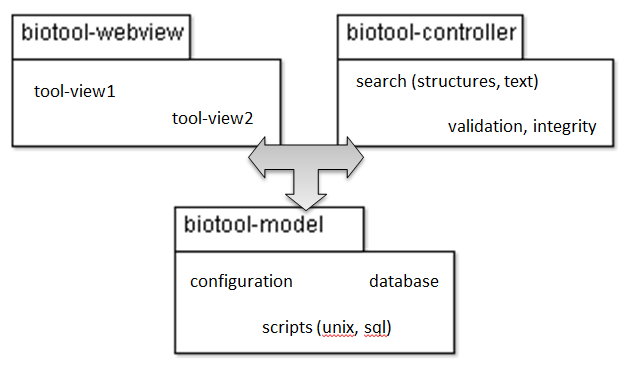
\includegraphics[width=\columnwidth]{SimpleClassDiagram.png}%
%\caption{The functional units from the biotool architecture can be grouped together in a refactoring process, putting similar functions together. The result may resemble a Model-View-Controller architecture.}%
%\label{fig-not-spaghetti}%
%\end{figure}

\section*{Conclusion}

Effective software engineering is a challenge in any enterprise, but may be even more so in the research context. Among other reasons, the research context can encourage a rapid turnover of staff, with the result that knowledge about legacy systems is lost. There can be a shortage of software engineering-specific training, and ``publish or perish'' culture may incentivise taking shortcuts. 

The recommendations above give a brief introduction to established best practices in software engineering that may serve as a useful introduction and reference. Some of these recommendations may be debated in some contexts, but nevertheless are important to understand and master. To learn more, Table~\ref{tab:learnmore} lists some additional online and educational resources. 

%%%%%%%%%%%%%%%%%%%%%%%%%%%%%%%%%%%%%%%%%%%%%%
%%                                          %%
%% Backmatter begins here                   %%
%%                                          %%
%%%%%%%%%%%%%%%%%%%%%%%%%%%%%%%%%%%%%%%%%%%%%%

\begin{backmatter}

\section*{Competing interests}
  The authors declare that they have no competing interests.

\section*{Author's contributions}
  JH prepared the initial draft. All authors contributed to, and have read and approved, the final version. 

\section*{Acknowledgements}
  This commentary is based on a presentation given by JH at a workshop on Software Engineering held at the 2014 annual Metabolomics conference in Tsuruoka, Japan. The authors would like to thank Saravanan Dayalan for organising the workshop and giving JH the opportunity to present. We would furthermore like to thank Robert P. Davey and Chris Mungall for their careful and extremely helpful reviews of an earlier version of this manuscript. 
%%%%%%%%%%%%%%%%%%%%%%%%%%%%%%%%%%%%%%%%%%%%%%%%%%%%%%%%%%%%%
%%                  The Bibliography                       %%
%%                                                         %%
%%  Bmc_mathpys.bst  will be used to                       %%
%%  create a .BBL file for submission.                     %%
%%  After submission of the .TEX file,                     %%
%%  you will be prompted to submit your .BBL file.         %%
%%                                                         %%
%%                                                         %%
%%  Note that the displayed Bibliography will not          %%
%%  necessarily be rendered by Latex exactly as specified  %%
%%  in the online Instructions for Authors.                %%
%%                                                         %%
%%%%%%%%%%%%%%%%%%%%%%%%%%%%%%%%%%%%%%%%%%%%%%%%%%%%%%%%%%%%%

% if your bibliography is in bibtex format, use those commands:
\bibliographystyle{bmc-mathphys} % Style BST file
\bibliography{bmc_article}      % Bibliography file (usually '*.bib' )

% or include bibliography directly:
% \begin{thebibliography}
% \bibitem{b1}
% \end{thebibliography}

%%%%%%%%%%%%%%%%%%%%%%%%%%%%%%%%%%%
%%                               %%
%% Figures                       %%
%%                               %%
%% NB: this is for captions and  %%
%% Titles. All graphics must be  %%
%% submitted separately and NOT  %%
%% included in the Tex document  %%
%%                               %%
%%%%%%%%%%%%%%%%%%%%%%%%%%%%%%%%%%%

%%
%% Do not use \listoffigures as most will included as separate files

\section*{Figures}

\begin{figure}[h!]%
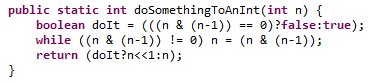
\includegraphics[width=\columnwidth]{code-snippet.png}%
\caption{An example of incomprehensible code: What does this code actually do? It contains a bug; is it easy to spot?}%
\label{fig-incomprehensible}%
\end{figure}

\begin{figure}[h!]%
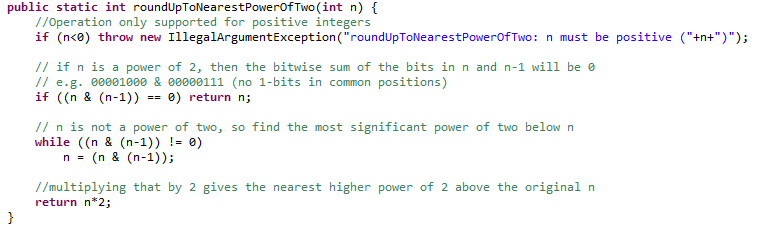
\includegraphics[width=\columnwidth]{code-snippet-fixed.png}%
\caption{This code peforms the same function, but is written more clearly.}%
\label{fig-comprehensible}%
\end{figure}

\begin{figure}[h!]%
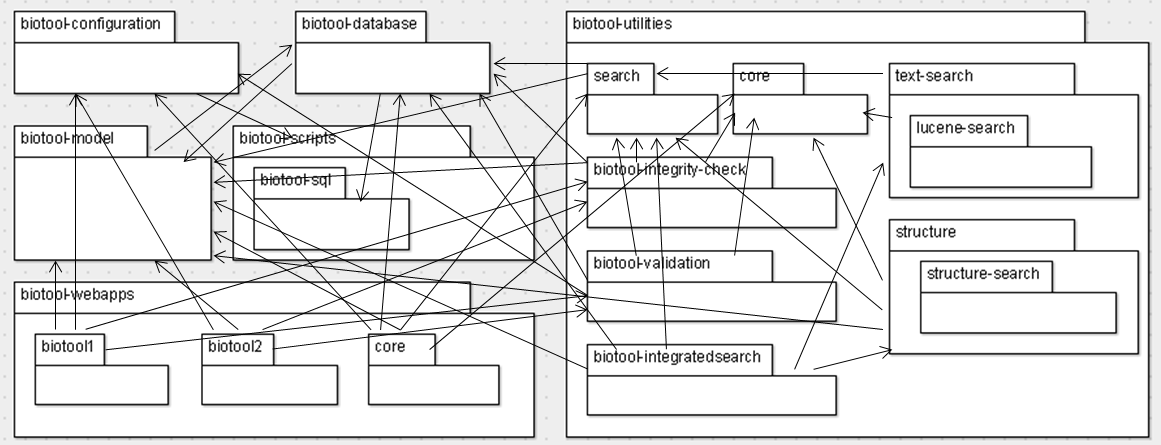
\includegraphics[width=\columnwidth]{ComplexClassDiagram.png}%
\caption{An unhealthy module design for `biotool` with multiple interdependencies between different packages. An addition of functionality to the system (such as supporting a new field) requires updating the software in many different places. Refactoring into a simpler architecture would improve maintainability.}%
\label{fig-spaghetti}%
\end{figure}

\begin{figure}[h!]%
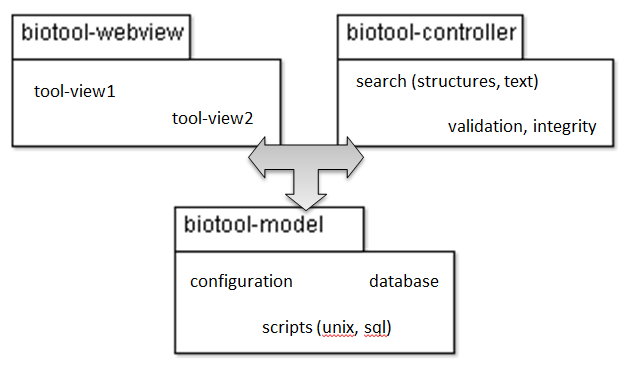
\includegraphics[width=\columnwidth]{SimpleClassDiagram.png}%
\caption{The functional units from the biotool architecture can be grouped together in a refactoring process, putting similar functions together. The result may resemble a Model-View-Controller architecture.}%
\label{fig-not-spaghetti}%
\end{figure}

%%%%%%%%%%%%%%%%%%%%%%%%%%%%%%%%%%%
%%                               %%
%% Tables                        %%
%%                               %%
%%%%%%%%%%%%%%%%%%%%%%%%%%%%%%%%%%%

%% Use of \listoftables is discouraged.
%%
\section*{Tables}
\begin{table}[h!]
\caption{Further reading. This table lists additional online resources where the interested reader can learn more about good practice in software engineering.}
\label{tab:learnmore}
      \begin{tabular}{| p{5cm} | p{5cm} |}
        \hline
        Description & URL \\ \hline 
        Software Carpentry: scientific computing skills, learn online or in face-to-face workshops & http://software-carpentry.org/ \\
        Learn about how to write maintainable code through counter-examples & http://www.thc.org/root/phun/unmaintain.html \\ \hline
      \end{tabular}
\end{table}

%%%%%%%%%%%%%%%%%%%%%%%%%%%%%%%%%%%
%%                               %%
%% Additional Files              %%
%%                               %%
%%%%%%%%%%%%%%%%%%%%%%%%%%%%%%%%%%%

%\section*{Additional Files}
%  \subsection*{Additional file 1 --- Sample additional file title}
%    Additional file descriptions text (including details of how to
%    view the file, if it is in a non-standard format or the file extension).  This might
%    refer to a multi-page table or a figure.

  %\subsection*{Additional file 2 --- Sample additional file title}
   % Additional file descriptions text.


\end{backmatter}
\end{document}
